\section{Experiments}\label{sec:expts}

\subsection{Datasets}
\begin{table*}[h]
\small
  \begin{tabularx}{\textwidth}{ p{2.0cm} | p{0.6cm} p{1.2cm} p{1.2cm} X }
  Dataset & Pairs & Arguments & Undecided & Dataset properties \\\hline\hline
  Toy Datasets & 4-13 & 4-5 & 0-9 & Synthetic pairwise labels
  \newline Arguments sampled at random from UKPConvArgStrict\\  
  \hline\emph{UKPConvArg-Strict} &
  11642 &
  1052 & 
  0 &
  Combine crowdsourced pairwise labels with MACE \newline
  Gold labels are $\ge 95\%$ most confident MACE labels \newline
  Discard arguments marked as equally convincing \newline
  Discard conflicting preferences \\
  \hline\emph{UKPConvArg-Rank} &
  16081 &
  1052 &
  3289 &
  Combine crowdsourced pairwise labels with MACE \newline
  Gold labels are $\ge 95\%$ most confident MACE labels \newline
  PageRank run on each topic to produce gold rankings \\  
  \hline\emph{UKPConvArg-CrowdSample} &
  16927 & 
  1052 &
  3698 &
  One original crowdsourced label per pair\newline
  PageRank run on each topic to produce gold rankings \newline
  Labels for evaluation from UKPConvArgStrict/UKPConvArgRank
  \end{tabularx}
  \caption{\label{tab:expt_data} Summary of datasets, showing the different steps used to produce each Internet argument dataset.}
\end{table*}
We first use toy datasets to illustrate the behavior of several different methods (described below).
Then, 
we analyze the scalability and performance of our approach on datasets provided by Habernal and Gurevych~\shortcite{habernal2016argument},
which contain pairwise labels for arguments taken from online discussion forums.
The labels can have a value of $0$, meaning the annotator found the second argument in the pair more convincing,
$1$ if the annotator was undecided, or $2$ if the first argument was more convincing.
To test different scenarios, different pre-processing steps were used to produce the
three \emph{UKPConvArg*} datasets shown in Table \ref{tab:expt_data}.
\emph{UKPConvArgStrict} and \emph{UKPConvArgRank} were cleaned to remove disagreements between annotators, hence can be considered to be \emph{noise-free}.
 \emph{UKPConvArgCrowdSample} is used to evaluate performance with noisy crowdsourced data 
including conflicts and undecided labels, and to test the suitability of our method for active learning
to address the cold-start problem in domains with no labeled data.
For these datasets, we perform 32-fold cross validation, where
%, using 31 folds for training and one for testing. 
each fold corresponds to one of 16 controversial topics, and one of two stances for that topic.
 
\subsection{Method Comparison}

\begin{figure*}
\centering
\subfloat[no cycle]{
  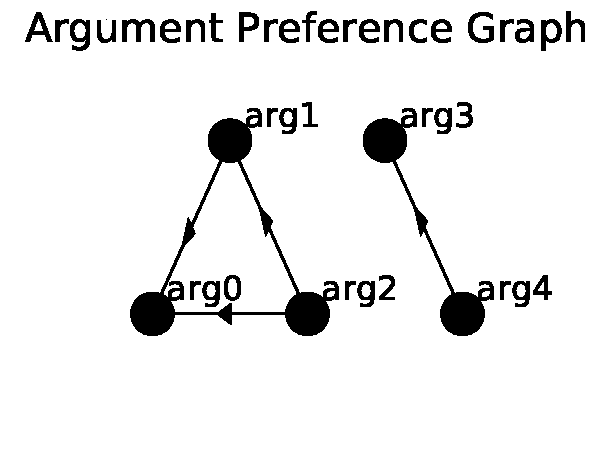
\includegraphics[width=.35\columnwidth, clip=True, trim=30 50 20 48]{figures/cycles_demo/no_cycle/arggraph_arg_graph}
}
\subfloat[single cycle]{
  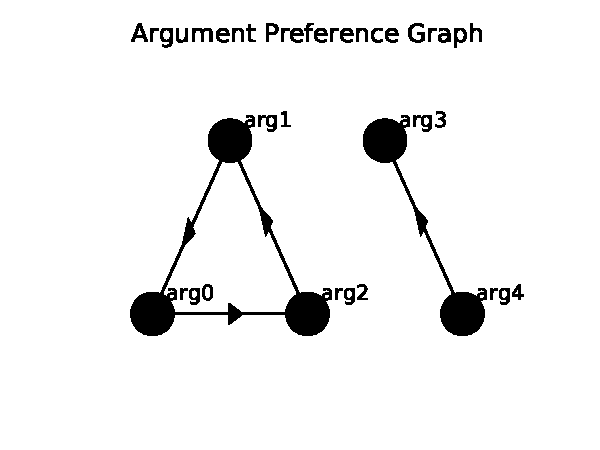
\includegraphics[width=.35\columnwidth, clip=True, trim=30 50 20 48]{figures/cycles_demo/simple_cycle/arggraph_arg_graph}
}
\subfloat[double cycle]{
  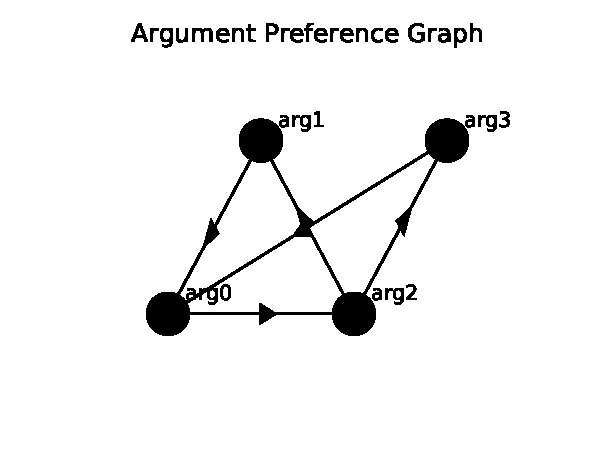
\includegraphics[width=.37\columnwidth, clip=True, trim=20 50 20 48]{figures/cycles_demo/double_cycle/arggraph_arg_graph}
}
\subfloat[no cycle + 9 undecided prefs.]{
  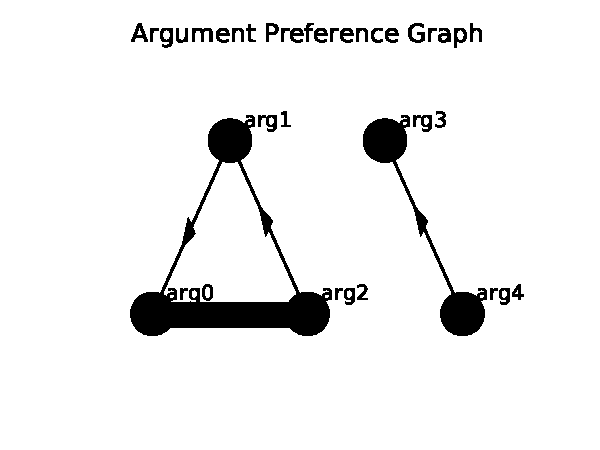
\includegraphics[width=.5\columnwidth, clip=True, trim=-30 50 -30 48]{figures/cycles_demo/undecided/arggraph_arg_graph}
}
\caption{Argument preference graphs for each scenario. Arrows point to the preferred argument.}
\label{fig:arg_graph}
\end{figure*}
\begin{figure*}
\centering
\subfloat[no cycle]{
  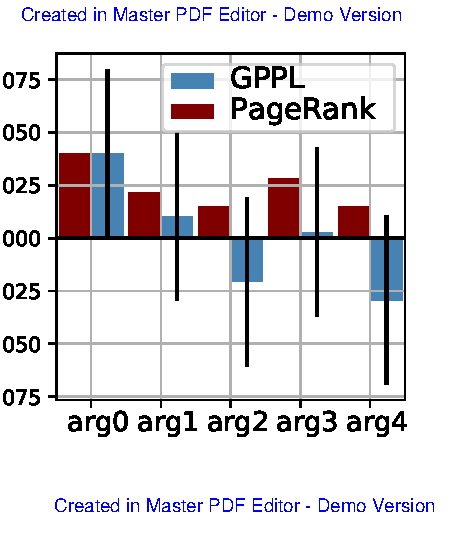
\includegraphics[width=.40\columnwidth, clip=True, trim=20 47 10 25]{figures/cycles_demo/no_cycle/PageRank_scores}
}
\subfloat[single cycle]{
  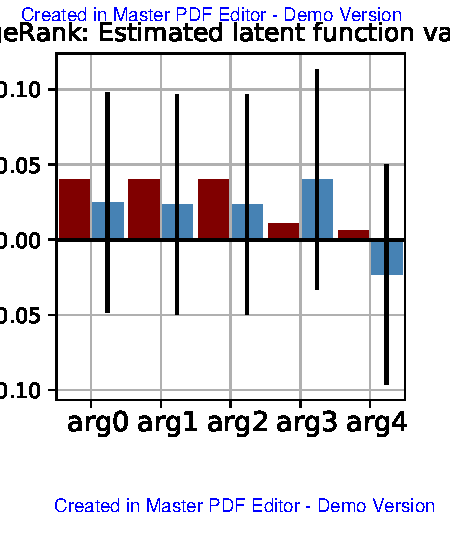
\includegraphics[width=.40\columnwidth, clip=True, trim=20 47 10 22]{figures/cycles_demo/simple_cycle/PageRank_scores}
}
\subfloat[double cycle]{
  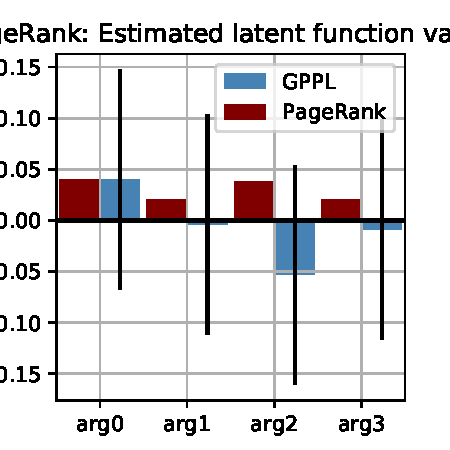
\includegraphics[width=.40\columnwidth, clip=True, trim=20 47 10 22]{figures/cycles_demo/double_cycle/PageRank_scores}
}
\subfloat[9 undecided]{
  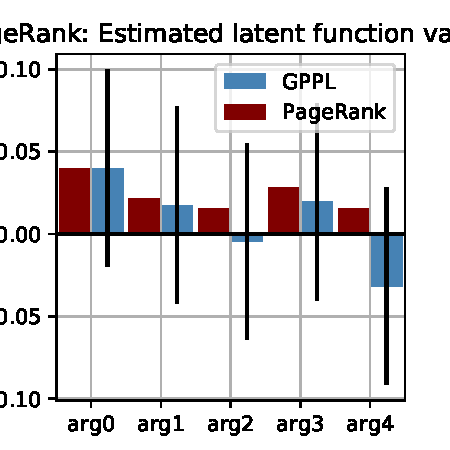
\includegraphics[width=.40\columnwidth, clip=True, trim=20 47 10 22]{figures/cycles_demo/undecided/PageRank_scores}
  \label{fig:ugraph}
}
\caption{Mean scores over 25 repeats. Bars for GPPL show standard deviation of convincingness function posterior.}
\label{fig:scores}
\end{figure*}
Our two tasks are \emph{ranking} arguments by convincingness and  
\emph{classification} of pairwise labels to predict which argument is more convincing. 
For both tasks, our proposed GPPL method is trained using the pairwise labels for the training folds.
We rank arguments by their expected convincingness, $\mathbb{E}[f(\mathbf{x}_i)]\approx \hat{f}(\mathbf {x_i})$ for each argument $i$ with feature vector $\mathbf{x}_i$, under the approximate posterior $q(\mathbf f)$
output by our SVI algorithm.
We obtain classification probabilities using Equation \ref{eq:plphi} but 
accommodate the posterior covariance, $\mathbf C$, of $\mathbf f$, by replacing $z$ with $\hat{z} = (\hat{f}(\mathbf x_i) - \hat{f}(\mathbf x_j)) / \sqrt{2 + C_{ii} + C_{jj} - C_{ij} - C_{ji}}$.
We tested the sensitivity of GPPL to the choice of seed values for K-means++ by training the model on the same $31$ folds of UKPConvArgStrict $20$ times, each with a different random seed, then testing on the remaining fold.
The resulting accuracy had a standard deviation of $0.03$. 
In the following experiments, all methods were initialized and trained once for each fold of each experiment.

We compare GPPL to an SVM with radial basis function kernel, 
and a bi-directional long short-term memory network (BiLSTM),
with $64$ output nodes in the core LSTM layer. 
The SVM and BiLSTM were tested by Habernal and Gurevych~\shortcite{habernal2016argument} and are available in our software repository.
To apply SVM and BiLSTM to the classification task, we concatenate the feature vectors of each pair of arguments and train on the pairwise labels.
For ranking, PageRank is first applied to arguments in the training folds to obtain scores from the pairwise labels,
which are then used to train the SVM and BiLSTM regression models.

% This gives standard deviations of a few percent. However, since we have 32 samples in each mean, what is the expected noise level this will introduce? 
% This ought to be accounted for in the p-values computation -- wilcoxon doesn't have a way to input known noise levels and cares only about the order of pairs of results, not
% their magnitude. 
% Should we mention the variation due to K-means initialization at all? 
% for fold 0, embeddings
% Mean ACC across reps: 0.508579
% Mean AUC across reps: 0.503808
% Mean CEE across reps: 1.272462
% Var ACC across reps: 0.002578
% Var AUC across reps: 0.005331
% Var CEE across reps: 0.062024
% Mean ACC across reps: 0.731000
% Mean AUC across reps: 0.795236
% Var ACC across reps: 0.004581
% Var AUC across reps: 0.006719

% for fold 3, embeddings
% Mean ACC across reps: 0.800000
% Mean AUC across reps: 0.875666
% Mean CEE across reps: 0.480064
% Var ACC across reps: 0.001174
% Var AUC across reps: 0.001783
% Var CEE across reps: 0.013538

% for fold 8, both
% Mean ACC across reps: 0.793578
% Mean AUC across reps: 0.881035
% Mean CEE across reps: 0.436018
% Var ACC across reps: 0.000141
% Var AUC across reps: 0.000072
% Var CEE across reps: 0.000257

% this gives: 0.012 accuracy with both, 0.008 for AUC, 0.016 for CEE


As a Bayesian alternative to GPPL, 
we test a Gaussian process classifier (\emph{GPC}) for the classification task 
by concatenating the feature vectors of arguments in the same way as the SVM classifier.
We also evaluate a non-Bayesian approach that infers function values using the 
same pairwise preference likelihood (\emph{PL}) as GPPL
(Equation \ref{eq:plphi}), 
but uses them to train an SVM regression model instead of a GP. 
We refer to this method as \emph{PL+SVR}.

We use two sets of input features. The \emph{ling} feature set contains $32,010$ linguistic features,  
including unigrams, bigrams, parts-of-speech (POS) n-grams, production rules,
ratios and counts of word length, punctuation and verb forms,
dependency tree depth, named entity type counts,
readability measures, sentiment scores, and spell-checking.
The \emph{GloVe} features are word embeddings with 300 dimensions. Both feature sets were
developed by Habernal and Gurevych~\shortcite{habernal2016argument}.
%As word embeddings may contain complementary semantic information to linguistic features, we evaluate with each feature set and a 
We also evaluate a combination of both feature sets, \emph{ling + GloVe}.
To create a single embedding vector per argument as input for GPPL,
we take the mean of individual word embeddings for tokens in the argument.
We also tested skip-thoughts~\cite{kiros2015skip} and Siamese-CBOW~\cite{kenter2016siamesecbow} 
with GPPL on UKPConvArgStrict and UKPConvArgRank, both with MLII optimization and the median heuristic,
 both alone and combined with \emph{ling}. 
However, we found that mean GloVe embeddings produced substantially better performance in all tests.
To input the argument-level \emph{ling} features to BiLSTM, we extend the network by adding a dense layer with $64$ nodes. 

We set the GPPL hyper-parameters $a_0=2$ and $b_0=200$ by comparing
training set performance on UKPConvArgStrict and UKPConvArgRank against $a_0=2$, $b_0=20000$ and $a_0=2$, $b_0=2$.
The chosen prior is very weakly informative, favoring a moderate level of noise in the pairwise labels.
For the kernel function, $k_d$, we used the 
Mat\'ern $\frac{3}{2}$ function as it has been shown to outperform 
other commonly-used kernels, such as RBF, across a wide range of tasks~\cite{rasmussen_gaussian_2006}.
We defer evaluating other kernel functions to future work.
To set length-scales, $l_d$, we compare the median heuristic (labeled ``medi.")
with MLII optimization using an L-BFGS optimizer (``opt."). Experiment 2 shows how
the number of inducing points, $M$, can be set to trade off speed and accuracy. 
Following those results, we set $M=500$ for Experiments 3, 4 and 5 and $M=N$ for the toy dataset in Experiment 1.

\subsection{Experiment 1: Toy Data}

\begin{figure}
\centering
\captionsetup[subfloat]{labelformat=empty}
\subfloat[\;no cycle]{
  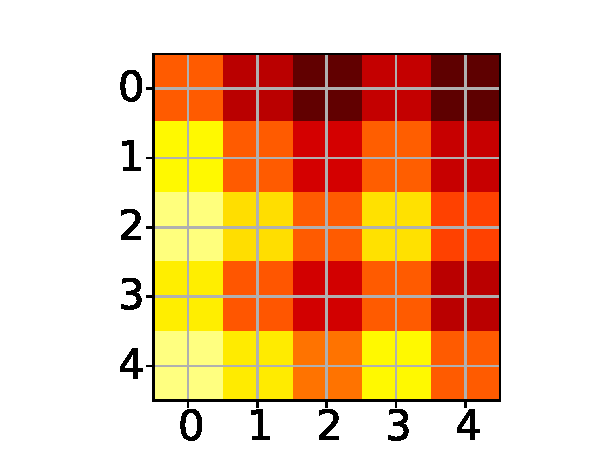
\includegraphics[width=.22\columnwidth, clip=True, trim=58 20 47 24]{figures/cycles_demo2/no_cycle/GPPL_probas}
}
\subfloat[single cycle]{
  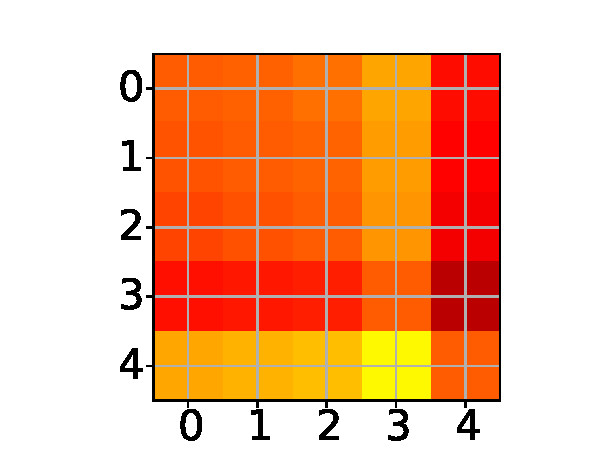
\includegraphics[width=.205\columnwidth, clip=True, trim=70 20 48 24]{figures/cycles_demo2/simple_cycle/GPPL_probas}
}
\subfloat[double cycle]{
  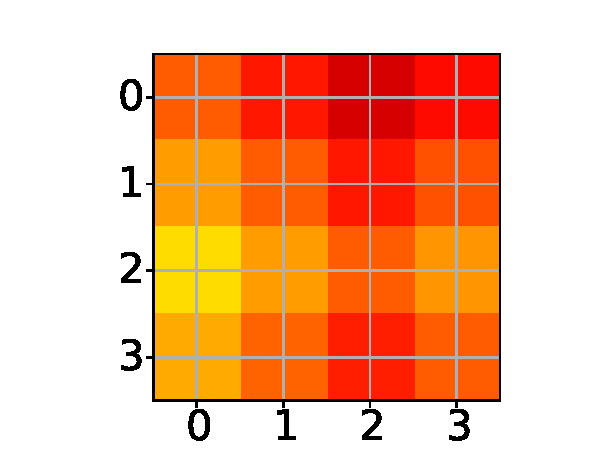
\includegraphics[width=.205\columnwidth, clip=True, trim=70 20 48 24]{figures/cycles_demo2/double_cycle/GPPL_probas}
}
\subfloat[9 undecided\;\;\;\;\;]{
  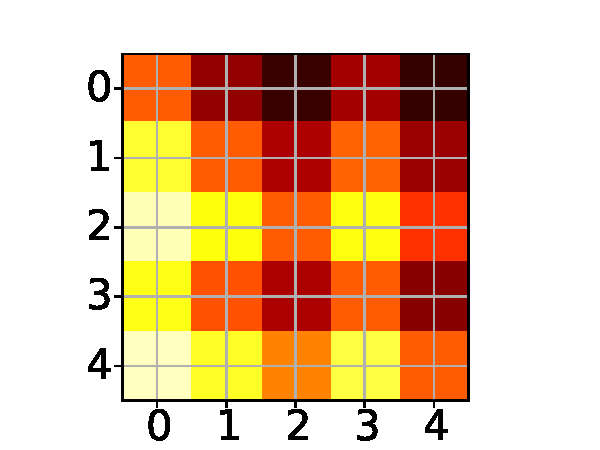
\includegraphics[width=.278\columnwidth, clip=True, trim=55 20 4 20]{figures/cycles_demo2/undecided/GPPL_probas}
}\\[-12pt]
\subfloat[]{
  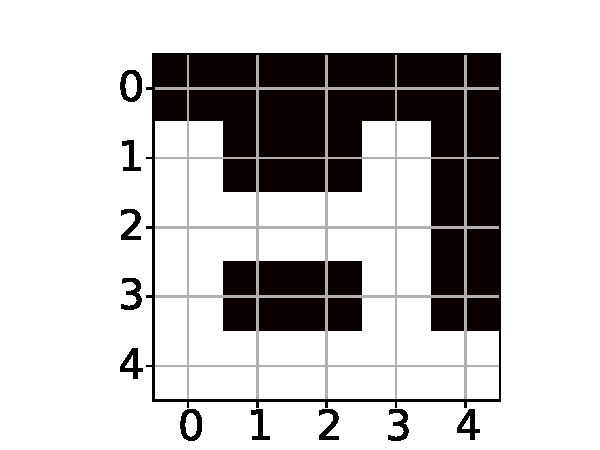
\includegraphics[width=.22\columnwidth, clip=True, trim=58 5 47 24]{figures/cycles_demo2/no_cycle/SVM_probas} 
}
\subfloat[]{
  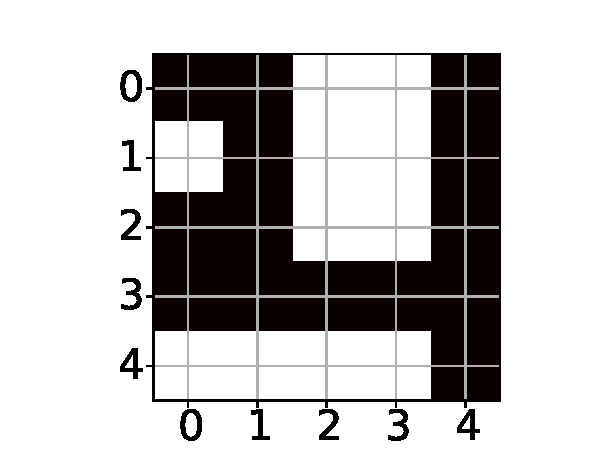
\includegraphics[width=.205\columnwidth, clip=True, trim=70 5 48 24]{figures/cycles_demo2/simple_cycle/SVM_probas} 
}
\subfloat[]{
  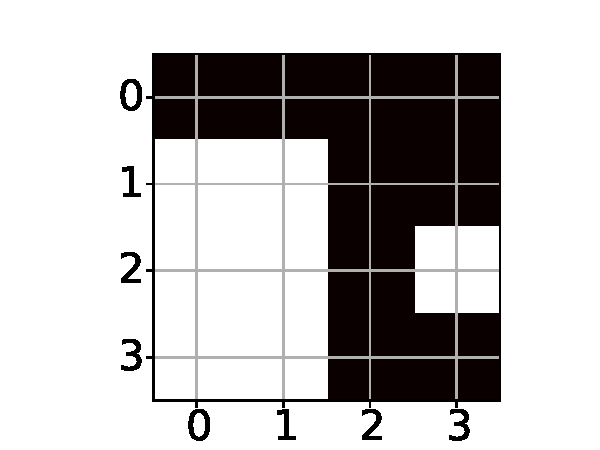
\includegraphics[width=.205\columnwidth, clip=True, trim=70 5 48 24]{figures/cycles_demo2/double_cycle/SVM_probas} 
}
\subfloat[]{
  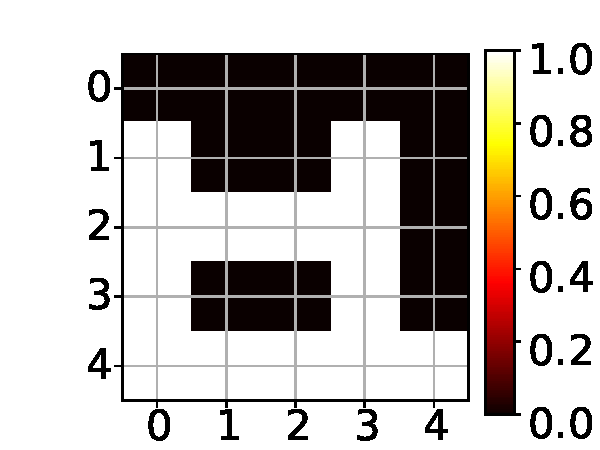
\includegraphics[width=.278\columnwidth, clip=True, trim=55 5 4 20]{figures/cycles_demo2/undecided/SVM_probas} 
}\\[-12pt]
\caption{Mean GPPL (top row) and SVM (bottom row) predictions over 25 repeats. Probability that the argument 
on the horizontal axis $\succ$ the argument on the vertical axis.}
\label{fig:cycle_demo_classification}
\end{figure}

To illustrate some key differences between GPPL, SVM and PageRank,
we simulate four scenarios, each of which contains arguments labeled \emph{arg0} to \emph{arg4}.  
In each scenario, we generate a set of pairwise preference labels according to the 
graphs shown in Figure \ref{fig:arg_graph}.
Each scenario is repeated 25 times: in each repeat, we select arguments at random from one fold of UKPConvArgStrict
then associate the mean GloVe embeddings for these arguments with the labels arg0 to arg4. 
We train GPPL, PageRank and the SVM classifier on the preference pairs shown in each graph and
predict ranks and pairwise labels for arguments arg0 to arg4.

\begin{figure*}[h]
\centering
\subfloat[Varying no. arguments in training set, GloVe features]{
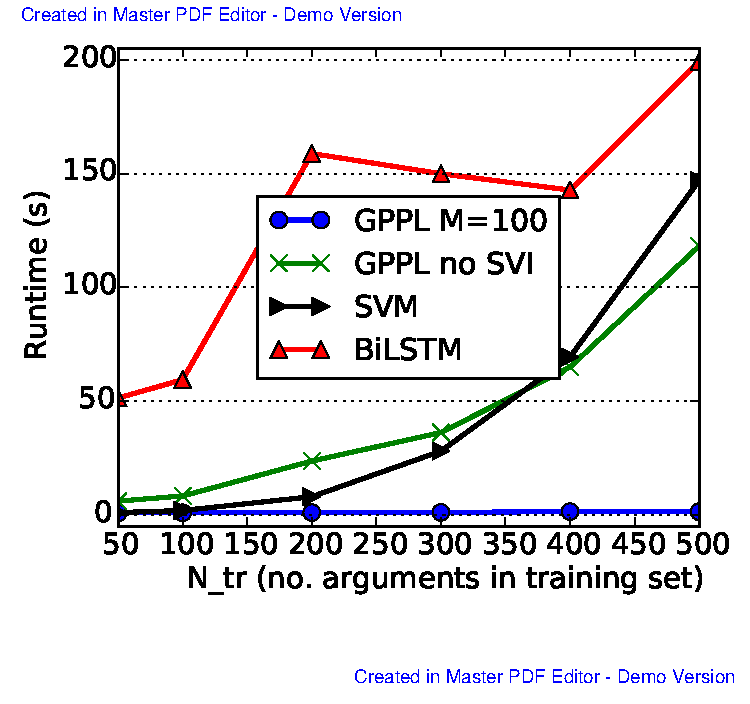
\includegraphics[width=0.62\columnwidth, clip=True, trim=12 18 0 13.5]{figures/scalability/num_arguments.pdf}
\label{fig:scale_N}
}
\hspace{0.1cm}
\subfloat[Varying no. ling+GloVe features, GPPL, medi., M=500]{
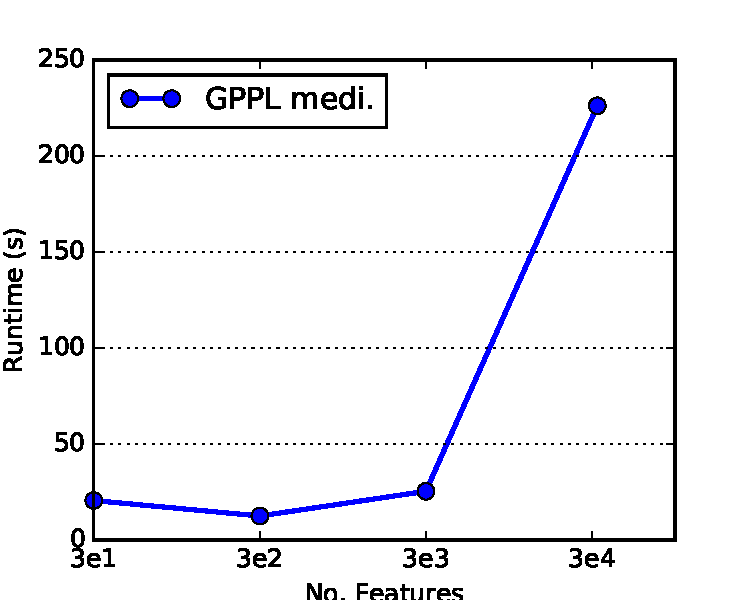
\includegraphics[width=0.55\columnwidth, clip=True, trim=20 47 0 20]{figures/scalability/num_features_gppl.pdf}
\label{fig:scale_dims}
}
\hspace{0.1cm}
\subfloat[Varying no. ling+GloVe features, long-running methods]{
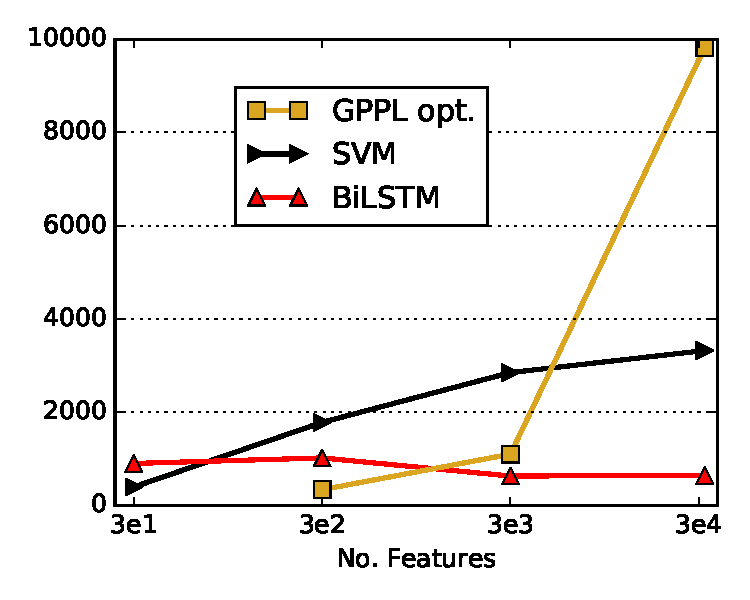
\includegraphics[width=0.58\columnwidth, clip=True, trim=0 58 10 20]{figures/scalability/num_features_others.pdf}
\label{fig:scale_dims_others}
}
\caption{Runtimes for training+prediction on UKPConvArgStrict with different subsamples of data. Means over 32 runs. Note logarithmic x-axis for (b) and (c). }
\end{figure*} 
\begin{figure}[t]
\subfloat[33210 ling+GloVe features]{
\hspace{-1.5mm}
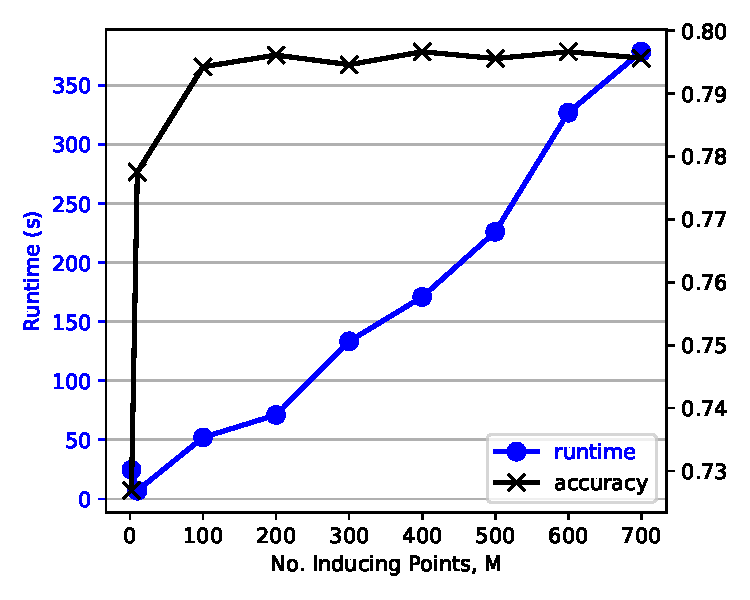
\includegraphics[width=0.49\columnwidth, clip=True, trim=4 40 13 12]{figures/scalability/num_inducing_32310_features.pdf}
\label{fig:scale_M_b}}
\subfloat[300 GloVe features]{
\hspace{-1.5mm}
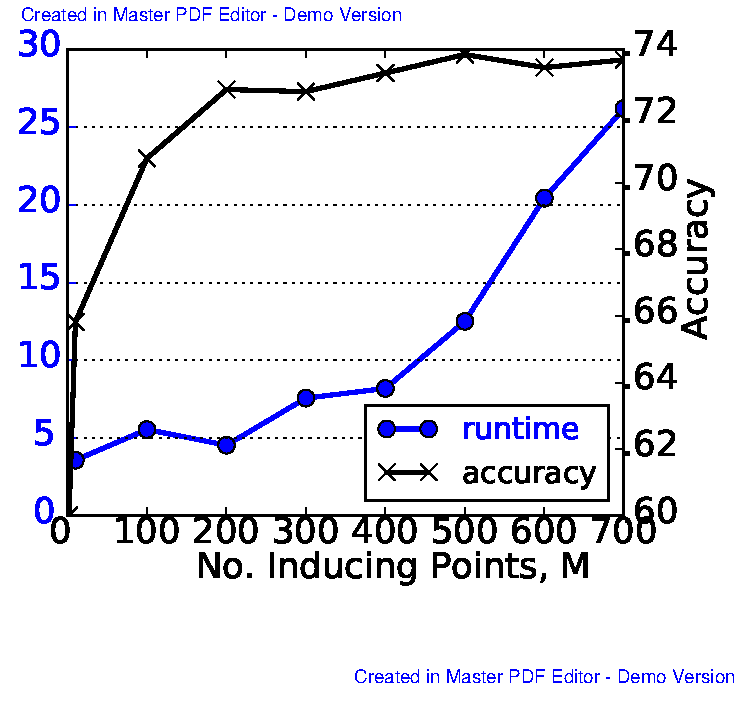
\includegraphics[width=0.48\columnwidth, clip=True, trim=8 40 17 12]{figures/scalability/num_inducing_300_features.pdf}
\label{fig:scale_M_a}}
\caption{Effect of varying $M$ on accuracy and runtime (training+prediction) of GPPL for UKPConvArgStrict.  Means over 32 runs.}
\label{fig:scale_M}
\end{figure}
In the  ``no cycle" scenario, 
arg0 is preferred to both arg1 and arg2, which is reflected in the scores predicted by PageRank and GPPL in Figure \ref{fig:scores}. However, arg3 and arg4 are not connected to the rest of the graph, and PageRank and GPPL score them differently. 
Figure \ref{fig:cycle_demo_classification} shows how GPPL provides less confident classifications for pairs that were not yet observed, e.g. arg2 $\succ$ arg4, in contrast with the discrete classifications of the SVM.

The next scenario shows a ``single cycle" in the preference graph.
Both PageRank and GPPL produce equal values for the arguments in the cycle (arg0, arg1, arg2). PageRank assigns lower scores to both arg3 and arg4 than the arguments in the cycle, 
while GPPL more intuitively gives a higher score to arg3, which was preferred to arg4. 
SVM predicts that arg0 and arg1 are preferred over arg3, 
although arg0 and arg1 are in a cycle so there is no reason to prefer them. 
GPPL, in contrast,  weakly predicts that arg3 is preferred.

The ``double cycle" scenario contains two paths from arg2 to arg0, via arg1 or arg3, and one conflicting
preference arg2 $\succ$ arg0. 
GPPL scores the arguments as if the single conflicting preference, arg2 $\succ$ arg0, 
is less important than the two parallel paths from arg2 to arg0. 
In contrast, PageRank gives high scores to both arg0 and arg2.
The classifications by GPPL and SVM are similar, but GPPL produces more uncertain 
predictions than in the first scenario due to the conflict.

Finally,  Figure \ref{fig:ugraph} shows the addition of $9$ undecided labels to the ``no cycle" scenario, indicated by 
undirected edges in Figure \ref{fig:arg_graph}, to simulate multiple annotators viewing the pair without being able to choose the most convincing argument.
The SVM and PageRank are unaffected as they cannot be trained using the undecided labels.
However, the GPPL classifications are less confident and the difference in GPPL scores between arg0 and the other arguments decreases, since GPPL gives the edge from arg2 to arg0 less weight.

In conclusion, GPPL appears to resolve conflicts in the preference graphs
more intuitively than PageRank, which was designed to rank web pages by 
importance rather than preference. 
In contrast to SVM, GPPL is able to account for cycles and undecided labels to soften its predictions.

\subsection{Experiment 2: Scalability}

We analyze empirically the scalability of the proposed SVI method for GPPL using the UKPConvArgStrict dataset.
Figure \ref{fig:scale_M} shows the effect of varying the number of inducing points, $M$, on the overall runtime and accuracy of the method. The accuracy increases quickly with $M$, and flattens out, suggesting there is little benefit to increasing  $M$ further on this dataset. 
The runtimes increase with $M$,  and are much longer with $32,310$ features than with 300 features.
The difference is due to the cost of computing the kernel, which is linear in $M$,
With only $300$ features, the Figure \ref{fig:scale_M_a} runtime appears polynomial, reflecting the 
$\mathcal{O}(M^3)$ term in the inference procedure. 

\begin{table*}
\small
  \begin{tabularx}{\textwidth}{ | l | X | X | X |  X |  X |  X |  X | X | X | X |}% X | X |}
  \hline
       &\multicolumn{2}{c|}{SVM}&\multicolumn{2}{c|}{BiLSTM}&\multicolumn{3}{c|}{GPPL median heuristic}&GPPL opt. & GPC & PL+ SVR\\\hline
       %& GPPL+, medi. & GPPL+, opt      \\\hline
       &ling &ling +GloVe &GloVe &ling +GloVe &ling &GloVe &\multicolumn{4}{c|}{ling +GloVe}\\\hline
\multicolumn{11}{| l |}{UKPConvArgStrict (pairwise classification)} \\   \hline       
Accuracy  &.78 & .79 &.76 & .77 &.78 &.71  &.79  & .80 & \textbf{.81} & .78\\%& .78 & .78     \\
ROC AUC   &.83 & .86 &.84 & .86 &.85 &.77  &.87  & .87 & \textbf{.89} & .85\\%& .86  &  .86    \\
CEE   &.52 & .47 &.64 & .57 &.51 &1.12  &.47  & .51 & \textbf{.43} & .51 \\%& .69  & .69   \\
\hline \multicolumn{11}{| l |}{UKPConvArgRank (ranking)} \\   \hline
Pearson's r      &.36 & .37 &.32 & .36 &.38 &.33  & \textbf{.45} &  .44 & - & .39 \\%& .40 &  .40   \\
Spearman's $\rho$&.47 & .48 &.37 & .43 &.62 &.44  &.65&  \textbf{.67} & - & .63\\% & .64 &  .64   \\
Kendall's $\tau$ &.34 & .34 &.27 & .31 &.47 &.31  &.49   &  \textbf{.50} & - & .47\\% & .49 &  .49   \\
\hline
  \end{tabularx}
  \caption{Performance comparison on UKPConvArgStrict and UKPConvArgRank datasets. }
  \label{tab:clean_results}
\end{table*}
We tested GPPL with both the SVI algorithm, with $M=100$ and $P_n=200$, and variational inference without inducing points or stochastic updates (labeled ``no SVI'') with different sizes of training dataset subsampled from UKPConvArgStrict. 
The results are shown in Figure \ref{fig:scale_N}. 
For GPPL with SVI, the runtime increases very little with dataset size, 
while the runtime with ``no SVI'' increases polynomially with training set size (both $N$ and $P$). 
At $N=100$, the number of inducing points is $M=N$ but the SVI algorithm is still faster due to the stochastic updates with $P_n=200 \ll P$ pairs.

Figure \ref{fig:scale_dims} shows the effect of the number of features, $D$, on runtimes.  
Runtimes for GPPL increase by a large amount with $D=32,310$,
 because the SVI method computes the kernel matrix, $K_{mm}$, with computational complexity $\mathcal{O}(D)$. 
 While $D$ is small, other costs dominate. 
We show runtimes using the MLII optimization procedure with GPPL in Figure \ref{fig:scale_dims_others}. 
Owing to the long computation times required, the procedure was limited to
a maximum of 25 iterations and did not terminate in fewer than 25 in any of the test runs. 
This creates a similar pattern to Figure \ref{fig:scale_dims} (approximately multiples of $50$).

We include runtimes for SVM and BiLSTM in Figures \ref{fig:scale_N} and
\ref{fig:scale_dims_others} to show their runtime patterns, but note that the runtimes reflect differences in implementations and system hardware.
Both SVM and GPPL were run on an Intel i7 quad-core desktop. For SVM we used LibSVM version 3.2, which could be sped up if probability estimates were not required.
BiLSTM was run with Theano 0.7\footnote{\url{http://deeplearning.net/software/theano/}} on an Nvidia Tesla P100 GPU. 
We can see in Figure \ref{fig:scale_dims_others} that the runtime for BiLSTM does
not appear to increase due to the number of features, while that of SVM increases sharply with $32,310$ features. 
In Figure \ref{fig:scale_N}, we observe the SVM runtimes increase polynomially with training set size. 

\subsection{Experiment 3: UKPConvArgStrict and UKPConvArgRank}
% \todo{statistical significance? paired Wilcoxon signed-rank test, GPPL ARD vs. SVM. }
% acc p-value of .043437
% auc p-value of .129870
% cee p-value of .000147. 
% Ranking: p-value of .000001
% p-value of .000001
% p-value of .000001
% 
% GPC to GPPL:
% p-value of .000012
% p-value of .000009
% p-value of .000001
% 
% GP+SVR to GPPL:
% p-value of .078799
% p-value of .056483
% p-value of .000171 --> differences mostly not significant
% p-value of .085377
% p-value of .045415
% p-value of .114077
%
% GPPL with combined features to ling
    %0.278126102583
%0.524930285518
%0.196971907599
We compare classification performance on UKPConvArgStrict  
and ranking performance on UKPConvArgRank. 
The results in Table \ref{tab:clean_results} show that when using \emph{ling} features,
GPPL produces similar accuracy and improves the area under the ROC curve (AUC) by $.02$ and cross entropy error (CEE) by $.01$.
AUC quantifies how well the predicted probabilities separate the classes,
while CEE quantifies the usefulness of the probabilities output by each method.
Much larger improvements can be seen in the ranking metrics. 
When GPPL is run with \emph{GloVe}, it performs worse than
BiLSTM for classification but improves the ranking metrics. 
Using a combination of features improves all methods, suggesting that embeddings and linguistic features contain complementary information. This improvement is statistically significant ($p \ll .01$ using two-tailed Wilcoxon signed-rank test) for SVM with all metrics except accuracy, for BiLSTM with AUC only, and for GPPL medi. with Pearson correlation only.

Optimizing the length-scale using MLII improves classification accuracy by 1\% over the median heuristic,
and significantly improves accuracy ($p=.043$) and AUC ($p=.013$) 
over the previous state-of-the-art, SVM \emph{ling}.
However, the cost of these improvements is that each fold required around 2 hours to compute instead of 
approximately 10 minutes on the same machine (Intel i7 quad-core desktop) using the median heuristic. 
The differences in all ranking metrics between GPPL opt. and SVM \emph{ling + GloVe} 
are statistically significant, with $p=.029$ for Pearson's $r$ and $p\ll.01$ for both 
Spearman's $\rho$ and Kendall's $\tau$.

GPC produces the best results on the classification task ($p<.01$ for all metrics compared to all other methods), 
indicating the benefits of a Bayesian approach over SVM and BiLSTM.
However, unlike GPPL, GPC cannot be used to rank the arguments.
The results also show that PL+SVR does not reach the same performance as GPPL, 
suggesting that GPPL may benefit from the Bayesian integration of a GP with the preference likelihood. 

\subsection{Experiment 4: Conflicting and Noisy Data}

\begin{table}
\small
  \begin{tabularx}{\columnwidth}{ | l | X | X | X | X | X |}\hline
% \multicolumn{6}{|l|}{UKPConvArgAll} \\   \hline
             & SVM & Bi-LSTM &GPPL medi.        &PL+ SVR     &GPC \\\hline
\multicolumn{6}{| l |}{Classification} \\   \hline             
% Acc:     &.71 &.73  & .77        &.75       &.76 \\
% AUC:          &.81 &.81  & .84        &.82       &.86 \\
% CEE:          &.56 &.53  & .49        &.52       &.50 \\
Acc          & .70 & .73 & \textbf{.77}        &.75       &.73 \\
AUC          & .81 & .81 & .84        &.82       & \textbf{.86} \\
CEE          & .58 & .55 & \textbf{.50}     &.55       &.53 \\\hline
\multicolumn{6}{| l |}{Ranking} \\   \hline             
Pears.       & .32 & .22 & \textbf{.35}        &.31       & - \\
Spear.       & .43 & .30 & .54        & \textbf{.55}       & - \\
Kend.        & .31 & .21 & \textbf{.40}        & \textbf{.40}       & - \\
%             &SVM ling & Bi-LSTM GloVe % removed these results as not needed
%Acc          &.70 &.73 
%AUC          &.81 &.80 
%CEE          &.58 &.54
%Pears.       &.18 &.26
%Spear.       &.17 &.20
%Kend.        &.12 &.13
\hline
  \end{tabularx}
  \caption{Performance comparison on UKPConvArgCrowdSample using ling+GloVe features.}
  \label{tab:noisy}
\end{table}
We use UKPConvArgCrowdSample to introduce noisy data
and conflicting pairwise labels
to both the classification and regression tasks, to test
the hypothesis that GPPL would best handle unreliable crowdsourced data.
The evaluation uses gold labels from UKPConvArgStrict and UKPConvArgRank for the test set.
The results in Table \ref{tab:noisy} show that all methods perform worse compared to 
Experiment 3 due to the presence of errors in the pairwise labels. 
Here, GPPL produces the best classification accuracy and cross-entropy error (significant with $p\ll.01$ compared to all other methods except accuracy compared to GP+SVR, for which $p=.045$), while GPC has the highest AUC ($p\ll.01$ compared to all except GP+SVR, which was not significant). 
Compared to UKPConvArgStrict, the classification performance of GPC, SVM and BiLSTM decreased more than that of GPPL.
These methods lack a mechanism to resolve conflicts in the preference graph, unlike GPPL and PL+SVR, which handle conflicts through the preference likelihood.  
PL+SVR again performs worse than GPPL on classification metrics, although its ranking performance is comparable. 
For ranking, GPPL again outperforms SVM and BiLSTM in all metrics (significant with $p\ll.01$ in all cases except for SVM with Pearson's correlation).

%Comparing both features to individual sets on this dataset... the only significant diffs are:    
%SVM, both vs. ling
%AUC 0.0175601092338
%CEE 0.028177011367

%BiLSTM both vs embeddings
%AUC 0.0726380522016
%SPEarman 0.0122223799995
%Kendall 0.00837537296597

\subsection{Experiment 5: Active Learning}

In this experiment, we hypothesized that GPPL provides more meaningful confidence estimates than SVM or BiLSTM,
which can be used to facilitate active learning in scenarios where labeled training data is expensive
or initially unavailable.
To test this hypothesis, we simulate an active learning scenario, in which an agent 
iteratively learns a model for each fold. Initially, $2$ pairs are chosen at random, then used to train the classifier. The agent then performs \emph{uncertainty sampling}~\cite{settles2010active} 
to select the $2$ pairs with the least confident classifications. 
The labels for these pairs are then added to the training set and 
used to re-train the model. We repeated the process until $400$ labels had been sampled. 

The result is plotted in Figure \ref{fig:active_learning}, showing that GPPL
reaches a mean accuracy of 70\% with only 100 labels, while SVM and BiLSTM do not reach the same performance given 400 labels. 
After 100 labels, the 
performance of BiLSTM decreases. It has previously been shown ~\cite{cawley2011baseline,guyon2011results,settles2010active} that uncertainty sampling sometimes causes accuracy to decrease. If the model overfits to a small dataset, 
it can mis-classify some data points with high confidence so that they are not selected and corrected by uncertainty sampling.  
The larger number of parameters in the BiLSTM may make it may more prone to overfitting with small datasets than SVM or GPPL. 
The Bayesian approach of GPPL aims to further 
reduce overfitting by accounting for parameter uncertainty.
The results suggest that GPPL may be more suitable than the alternatives in cold-start scenarios with small amounts of labeled data. 
\begin{figure}
\centering
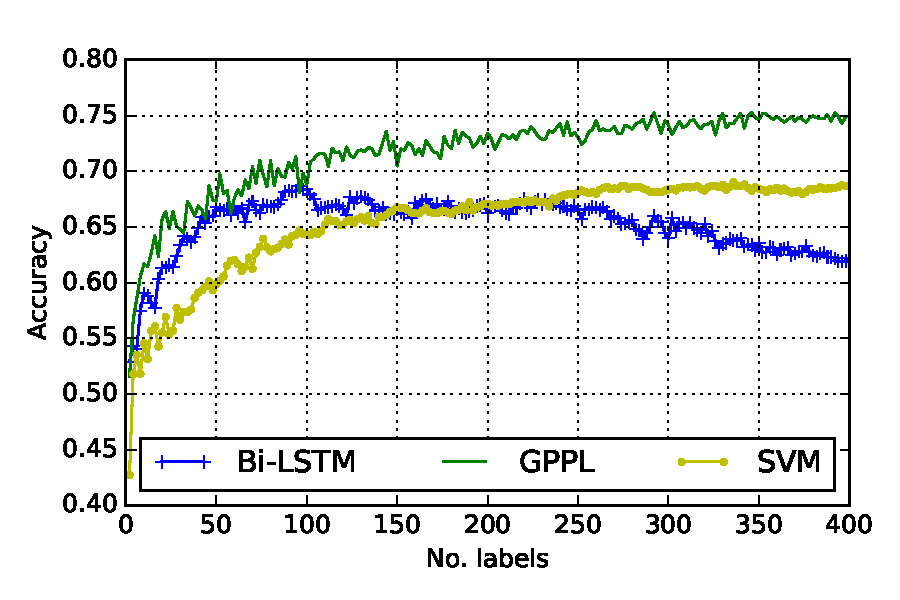
\includegraphics[width=0.9\columnwidth,trim=13 15 10 22.5,clip=true]{figures/active_learning_2/test_acc}
\caption{Active learning simulation showing mean accuracy of preference pair classifications over 32 runs.}
\label{fig:active_learning}
\end{figure}

\subsection{Relevant Feature Determination}

We now examine the length-scales learned by optimizing GPPL using MLII  
to identify informative features. 
A larger length-scale causes greater smoothing, 
implying that the feature is less relevant when predicting the convincingness function
than a feature with a small length-scale. 
Figure \ref{fig:boxplot} shows the distribution of length-scales for each category of
\emph{ling+GloVe} features, averaged over the folds in UKPConvArgStrict where MLII
optimization improved accuracy by $\>3\%$. The length-scales
were normalized by dividing by their median heuristic values, 
which were their initial values before optimization.
The widest distributions of length-scales are for the mean word embeddings and the ``other'' category.
A very large number of features have length-scales close to $1$,
which may mean that they are weakly informative, as their length-scales have not been increased,
or that there was insufficient data or time to learn their length-scales.
To limit computation time, the optimization algorithm was restricted to $25$ iterations, 
so may only have fully optimized features with larger gradients, 
leaving other features with normalized length-scales close to $1$.
 
Table \ref{tab:extreme_features} shows features with length-scales $<0.99$,
of which there are two production rule features and $18$ POS-n-gram features,
suggesting that the latter may capture more relevant aspects of grammar for convincingness. 
For n-grams, the relationship to convincingness may be topic-specific, 
hence they are not identified as important when the model is trained on $31$ different topics. 
%The n-grams with length-scales $<0.99$ may be indicative of the
%number of sentences -- it is possible very short arguments correlate with
%less convincing arguments.
The fact that MLII did not substantially shorten the length-scales for n-grams and POS n-grams 
corresponds to previous results ~\cite{persing2017can}, which found these feature sets less informative than other argument-related feature sets.
 
Table \ref{tab:extreme_features} also presents a breakdown of the ``other'' features into sentiment, ratio, count and NER features. 
The shortest length-scales are for sentiment features, pointing to a possible link between 
argumentation quality and sentiment. However, ``VeryPositive'' was the feature with
the largest length-scale, either because the median was a poor heuristic in this case or
because the feature was uninformative, perhaps because sarcastic statements can be confused with highly positive sentiment.
The short length-scale for the ``words $>6$ letters'' ratio suggest that some surface features may be informative,
despite previous work \cite{wei2016post} finding a set of surface features less informative than other feature sets. 
In this case, longer words may relate to more sophisticated and convincing arguments. 
% It is possible that continuing the optimization procedure for a larger number of steps would 
% identify large length-scales for other features that may be discarded. However, caution is 
% required to avoid overfitting to the training set during optimization~\cite{qi2004predictive}.
\begin{figure}[h]
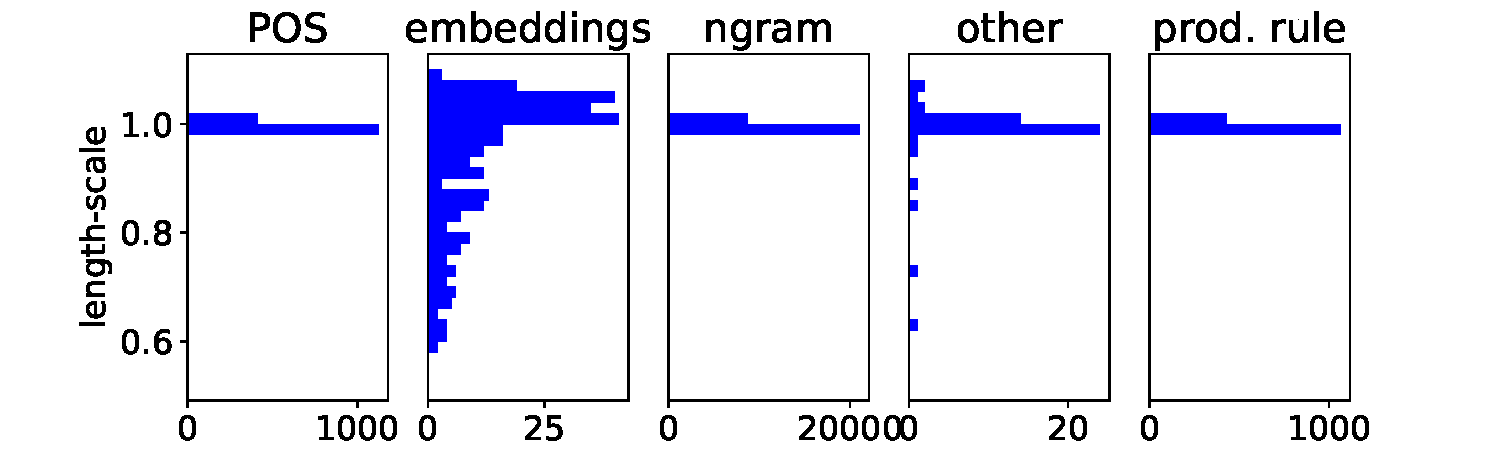
\includegraphics[width=\columnwidth, clip=True, trim=32 0 57 0]{figures/features2/boxplot}
\caption{Histograms of mean normalized length-scales on folds where MLII improved performance $>3\%$.}
\label{fig:boxplot}
\end{figure}
% old results pre bug-fix
% \begin{table}
% \small
%   \begin{tabularx}{\columnwidth}{l | X }
%   Feature & Ratio\\
%   \hline
%   ProductionRule-S-$>$ADVP,NP,VP,., & .466 \nonumber\\
%   Pos-ngram-PP-O-CARD & .477 \nonumber\\
%   Unigram-``safer", & .640 \nonumber\\
%   \hline
%   Bigram-``?"-``look" & 5.672 \nonumber\\
%   Unigram-``safest" & 8.673 \nonumber\\
%   Unigram-``safety" & 271.190 \nonumber\\
%   \hline
%   Embedding-dimension-19 & .610 \nonumber\\
%   \hline
%   Embedding-dimension-241 & 12.093 \nonumber\\
%   \end{tabularx}
%   \caption{Ratios of optimized to median heuristic length-scales: largest and smallest
%   ratios for linguistic features and word embeddings.}
%   \label{tab:extreme_features}
% \end{table}
\begin{table}[t]
\small
  \begin{tabularx}{\columnwidth}{l | X | r }
  Category & Feature & Length-scale\\
  \hline
  production rule & S$\to$NP,VP,.,	& 0.977\nonumber\\  
  production rule & S$\to$NP,VP,	& 0.988\nonumber\\  
  %ProductionRule & SBAR$\to$IN,S,	 & 0.992\nonumber\\   
  \hline
  POS-ngram & V-ADJ	& 0.950	\nonumber\\
  POS-ngram & PUNC-NN	& 0.974 \nonumber\\  
  POS-ngram & PR-PUNC	& 0.977	\nonumber\\
  POS-ngram & PP-V-PR	& 0.981\nonumber\\
  POS-ngram & NN-V-ADV	& 0.981\nonumber\\    
  \hline
  n-gram & ``.''	& 0.981\nonumber\\
  n-gram & ``to'' 	& 0.989\nonumber\\
  n-gram & ``in''	& 0.990\nonumber\\  
  \hline
  sentiment & Positive	& 0.636 \nonumber\\
  sentiment & VeryNegative	 & 0.842 \nonumber\\
  sentiment & Neutral	& 0.900 \nonumber\\
  sentiment & Negative & 0.967 \nonumber\\    
\emph{sentiment} & \emph{VeryPositive} & \emph{3.001} \nonumber \\% the only feature with very large lengthscale
\hline
  ratio & words $>$ 6 letters & 0.734 \nonumber\\
  ratio & SuperlativeAdj	& 0.943 \nonumber\\
  ratio & InterjectionRate	& 0.986 \nonumber\\
  ratio &	SuperlativeAdv	& 0.987 \nonumber\\
 \hline
  count & words $>$ 6 letters	& 0.983 \nonumber\\  
 \hline
  NER & Location & 0.990 \nonumber  
  \end{tabularx}
  \caption{Normalized length-scales for linguistic features learned using MLII. Shows mean values over folds with $>3\%$ improvement. Includes all values $<0.99$, except for POS n-grams (only smallest 5 of 18 shown).  }
  \label{tab:extreme_features}
\end{table}

\subsection{Error Analysis}

We compared the errors when using GPPL opt. with mean GloVe embeddings
and with linguistic features. We
manually inspected the $25$ arguments most frequently
mis-classified by GPPL \emph{ling} and correctly classified by GPPL \emph{GloVe}.
We found that GPPL \emph{ling} mistakenly marked several arguments 
as less convincing when they contained grammar and spelling errors but otherwise
made a logical point. 
In contrast, arguments that did not strongly take a side and did not contain 
language errors were often marked mistakenly as more convincing.

We also examined the $25$ arguments most frequently misclassified by GPPL \emph{GloVe} but not by GPPL \emph{ling}.
Of the arguments that GPPL \emph{GloVe} incorrectly marked as more convincing, 
$10$ contained multiple exclamation marks and all-caps sentences. 
Other failures were very short arguments and underrating arguments containing the term `rape'.
The analysis suggests that the different feature sets identify different aspects of convincingness.

% Notes on first paragraph:
% ling failed on:
% overrated: good grammar and structure but weak points?
% both; short and direct argument but not very thoughtful.
% both: seems well structured...
% both: seems to argue for middle ground rather than one side
% both: grammar/spelling errors but strong argument underneath?
% both: grammar/spelling errors but strong argument underneath?
% underrated: very specific example may seem off topic? 
% both: unclear points
% underrated: bad spelling but okay points
% underrated: very personal "I" language to make a good point
% mostly underrated: makes multiple points, some are quite extreme. 
% underrated: sounds quite personal "you" but strong argument.
% both: kind of doesn't try to convince strongly for one side although well written.
%  overrrated: doesn't address the main point although language is reasonable.
% mostly overrated: response to previous answer with no new points.
% underrated: contains '?' and 'you' a lot but makes a good point.
% overrated: language is reasonable, no mistakes, but doesn't clearly take a side.
% overrated: no obvious language indicators but doesn't address main point.
% underrated: lots of spelling mistakes hide the main point.
% mostly overrated: good language but doesn't really support or attack the point directly
% underrated argument with grammatical mistakes but possibly a good point?
% avoiding the argument/debate overrated
% illogical and quite emotional argument underrated
% personal/ad hom attack with 'crap' overrated -- but need to identify the username as such to know it  is a personal attack?
% obvious nonsense without proper words was overrated
%
% embeddings failed on:
%
% both: very short argument, unclear why ling features would help
% overrated: claims lack support
% overrated: spelling mistakes; doesn't address stance of the topic 
% underrated: very short; mean embedding could be an outlier?
% underrated: short
% underrated: no linguistic markers of a bad argument; unclear why embeddings a problem
%     mostly underrated; as above
% underrated: as above; perhaps the words such as 'rape' are associated in the embeddings
% with poor emotional arguments? Perhaps not the word 'rape' itself, but some of the related words in embedding space are common in bad arguments.
% underrated: no idea
% underrated: again mentions 'murder'
% mostly underrated: all caps; why underrated?
% underrated: sensible argument mentions 'personal' a lot
% underrated: very short; mentions wrong and right --> link to emotional arguments without evidence?
% overrated: very short and gives no argument; perhaps contains no bad argument embeddings but linguistic features such as word counts will show it up.
% overrated: mentions of 'dreamt'?
% underrated: no idea
% overrated: doesn't address main point; hard to see why ling would help
% underrated: no idea why; has no linguistic errors
% overrated: no idea; no idea why linguistic features help
% underrated: again maybe because of emotional topic of abortion; no linguistic problems
% overrated: very short sentence; no structure; lots of '!'
% overrated: grammatical errors, very short text that doesn't really make any point or provide any support
% overrated: nonsense detected by all caps
% overrated: very short, cannot really make a good point in that much text
% underrated: why this would beat any other argument is unclear; it's all caps and has lots of '!' too
% 
%  Problem is we don't see what they were misclassified against -- number of 
% misclassifications is too few to know if it is a general problem with that sentence.
% 
% which of these errors are resolved by combining? Pick out errors from either ling that
% were fixed with both; pick our errors from embeddings that were fixed with both.

% when comparing 'both' to 'ling', most of the errors that are made by embeddings
% no longer appear -- those with all caps and '!' have gone. Differences are few.
% seem to be that poorly written arguments continue to be mis-classified.
% with 'both' to embeddings, some of the errors that ling made have gone, e.g. including 'lol'. The remaining ones are mainly those with good superficial structure/correct grammar
% but covering emotional topics. Suggests need for better trade-off between semantics/deeper understanding and linguistic indicators such as good grammar.

% this analysis also shows whether the errors are due to epistemic uncertainty given the features (small difference in 
% similarities between false/true labeled items) or if better training data would help (larger difference between 
% false/true similarities). If GPPL handles the sparse data better, the difference should be reduced compared to SVM.
% the text below is good but the results are not really worth reporting...
%We next investigate whether the Bayesian approach is better able to handle sparsity in the training data. 
%Training data sparsity occurs when the training provides very few examples of arguments in some important regions of feature space, meaning  
% there are arguments in the test dataset that are not similar to any training arguments.
%For each fold, we computed the mean cosine similarity of each argument in the 
%test dataset to the arguments in the training dataset, which we refer to as \emph{training similarity}.
%For UKPConvArgStrict, the mean training similarity for the arguments in pairs correctly classified by GPPL (ling + GloVe) was 694.63 and the mean for incorrectly classified arguments was 694.703. This suggests that training similarity is not a strong indicator of a correct
%prediction and training data sparsity does not appear to be a key source of error for GPPL
%in this dataset. In comparison, using  SVM,  
%the mean training similarity for correctly classified arguments
% was 694.72 against .     for incorrectly classified arguments, showing that 
% lower training data similarity corresponds to a more misclassified pairs. 
% This indicates that SVM was more affected by training data sparsity.
% However, the small difference in similarities indicates that sparsity was not a problem here?
% The lower similarity of correctly labeled arguments with GPPL suggests it is able to handle more outlying arguments correctly. 
%results: 
% using matern covariance to determine similarity:
% SVM: correctly classified pairs: 694.715334 (STD 3.251511), incorrectly classified pairs: 694.164449 (STD 3.809051). 
% So similarity to training data is higher for correct pairs.
% GPPL: correctly classified pairs: 694.625999 (STD 3.213874), incorrectly classified pairs: 694.703252 (STD 3.580148).
% with cosine similarity:
%SVM For all folds: mean total_sim for correctly classified pairs: .998826 (STD .021547)
%SVM For all folds: mean total_sim for incorrectly classified pairs: .998770 (STD .025875)
%GPPL For all folds: mean total_sim for correctly classified pairs: .998825 (STD .021434)
%GPPL For all folds: mean total_sim for incorrectly classified pairs: .998770 (STD .026505)
% Using max similarity rather than mean (most similar training point) gives similar results.
% So similarity to training data is actually higher for incorrect pairs; for correct pairs it is lower than for SVM. 
% Suggests that similarity to training data (not being outliers) is less important for GPPL.

To investigate the differences between our best approach, GPPL opt. \emph{ling + GloVe}, 
and the previous best performer, SVM \emph{ling}, 
we manually examined $40$ randomly chosen false classifications, where one of 
either  \emph{ling + GloVe} or SVM was correct and the other was incorrect. 
We found that both SVM and GPPL falsely classified arguments that were either very short or long and complex, suggesting deeper semantic or structural understanding of the argument may be required. However, SVM also made mistakes
where the arguments contained few verbs.
%We were not able to identify any common source of error for cases where both 
%methods produced errors. % required deeper semantic understanding and background knowledge of the topics involved
% to evaluate the validity of claims.
% Case 1: SVM right, GPPL wrong.
% underrated, short
% overrated, maybe SVM is right because it dislikes '!'
% underrated, less common language -- perhaps not learned?
% overrated, complex language
% underrated, short argument
% ...
% overrated, irrelevant but well written
% more long arguments with fairly sophisticated language and no obvious errors.
% some cases of arguments that do not take a strong position either way
% The number of errors are small -- could be noise rather than consistent problems with GPPL.
% Some arguments with mainly topic-specific words were misclassified by GPPL but not SVM.
%notable that there are lots of errors on the singapore topics
% Case 2: GPPL right, SVM wrong
% short arguments with few verbs
% long arguments with no obvious language errors and no emotional arguments.
% notable that lots of errors on the school uniform topics

We also compared the rankings produced by GPPL opt. (ling+GloVe), 
and SVM on UKPConvArgRank by examining the 20 largest deviations from the 
gold standard rank for each method. Arguments underrated by SVM and not GPPL often 
contained exclamation marks or common spelling errors (likely due to unigram or bigram features).
GPPL underrated short arguments with the ngrams ``I think", ``why?", and
``don't know", which were used as part of a rhetorical question
rather than to state that the author was uncertain or uninformed.
These cases may not be distinguishable by a GP given only \emph{ling + GloVe} features.
% Case 1: GPPL better, SVM worse
% svm underrated some arguments containing !, thankyou, lots of 'if'
% underrated: long argument, common spelling errors (unigrams usually correlated with bad arguments?), India, long and complex arguments, short arguments
% overrated: ('because' could be either over or underrated), mention of another website, 
% Hard to see pattern here because the arguments are very varied in length, grammatical standard; most are not using emotive terms.

% Case 2: SVM better, GPPL worse
% mistakes by GPPL: several short arguments containing "i think"... perhaps leading to a more neutral score than the other features suggest?
% 

% Case 3: GPPL's worst problems (including mistakes by SVM)
% an argument with lots of caps in was underrated
% argument with lots of short sentences (sometimes few verbs) is underrated. 
% underrated: "why?"
% underrated: "don't know" is a big indicator. These two suggest that the model needs a way to determine whether the "don't know" was used in a way that undermines the argument strength (admission of a lack of knowledge) or as a rhetorical device to say that an opposing viewpoint is nonsensical ("don't know why they would do x"). 

% Entropy for SVM correct/incorrect labels: .187555, 1.583709
% Entropy for GPPL correct/incorrect labels: .128872, 2.443407
% Shows better division between certain and uncertain predictions
An expected advantage of GPPL is that it provides more meaningful uncertainty estimates for tasks such as active learning. 
We examined whether erroneous classifications correspond to more uncertain predictions
with GPPL \emph{ling} and SVM \emph{ling}.
For UKPConvArgStrict, the mean Shannon entropy
of the pairwise predictions from GPPL 
was .129 for correct predictions and 2.443 for errors,
while for SVM, the mean Shannon entropy was  .188 for correct predictions and 
1.583 for incorrect.
With both methods, more uncertain (higher entropy) predictions correlate with more errors,
but the more extreme values for GPPL suggest that its output probabilities more 
accurately reflect uncertainty than those produced by the SVM.

% % the analysis below is possible only using the predictions for the training points; however we do not predict for
% % the provided training points?
% To judge whether the GPPL improvements in UKPConvArgCrowdSample are due to better
% handling of noisy labels, we examined whether annotations that disagreed with the 
% MACE gold label -- i.e. erroneous training labels -- led to erroneous predictions. 
% We chart the results of this error analysis in Table \ref{tab:noise_errors}.
% This shows that while arguments with erroneous training labels are more likely to 
% be incorrectly classified using both SVM and GPPL, the Bayesian approach is less susceptible
% to this error.
% \begin{table}
% \begin{tabularx}{\columnwidth}{| l | X | X | X | X | }
% \hline
% & \multicolumn{4}{c | }{\emph{Predictions}} \\
% & \multicolumn{2}{c|}{SVM} & \multicolumn{2}{c|}{GPPL} \\\hline
% \emph{Annotations}           & \emph{True} & \emph{False} & \emph{True} & \emph{False} \\
% Incorrect & & & &  \\
% Correct   & & & & \\
% \hline
% \end{tabularx}
% \caption{Coincidence of erroneous annotations and false predictions by pairwise classification methods.}
% \label{tab:noise_errors}
% \end{table}
